\documentclass{article}

\usepackage{graphicx} % Allows including images
\usepackage{stackengine}
\usepackage{scalerel}
\usepackage{xcolor}
\usepackage{geometry}
\usepackage{multicol}
\usepackage{listings}

\graphicspath{{./../img/}}
\renewcommand{\abstractname}{}
\renewcommand{\tt}[1]{\texttt{#1}}

\newcommand\dangersign[1][2ex]{%
  \renewcommand\stacktype{L}%
  \scaleto{\stackon[1.3pt]{\color{red}$\triangle$}{\tiny !}}{#1}%
}

\newcommand{\warn}[1]{\begin{center}
\begin{tabular}{ c  p{12cm} }
\dangersign[22pt] & \vspace{-0.6cm} #1
\end{tabular}
\end{center}}

\geometry{
 a4paper,
 left=30mm,
 right=30mm,
 top=30mm,
 bottom=30mm
 }

\lstset{language=Python,
		commentstyle=\color{gray},
		keywordstyle=\color{blue},
		numberstyle=\color{yellow},
		stringstyle=\color{purple}
}


\title{\texttt{theia} \\ \quad \\A 3D Gaussian Beam Tracer for Gravitational Interferometers\\ \quad \\ \begin{small} Version 0.1.3 \end{small} \\ \quad \\ \textit{User Guide}}

\author{Rapha\"el Duque}

\begin{document}

\maketitle

\begin{abstract}
\tt{theia} is a command line program and Python library for 3D Gaussian beam tracing. It supports many different types of optical components, general 3D placing and orientation of these components and general astigmatic Gaussian beams, among other features. It allows the 3D visualization of the optical simulation by writing a CAD file read by the free software \tt{FreeCAD}. \tt{theia} was developed at the Optics Group of the Virgo gravitational observatory in Cascina, Italy. For more information on the Theia Project, surf to \tt{http://theia.hopto.org}.

This document is a user's guide to the \texttt{theia} command line tool. It gives the information concerning the installation instructions, the usage and the input and output of \texttt{theia} necessary to operate the program from the command line. It also provides a short introduction to the \tt{theia} library API. For more details on the \texttt{theia} Python library, please refer to the API Guide provided along with this User Guide, or go to \tt{http://theia.hopto.org/docs/html/index.html} for the online API guide.
\end{abstract}


\tableofcontents
\newpage


\section{\texttt{theia} Quick Start}
For a quick start of \tt{theia} once you are in the project repository, install \tt{theia} locally with \texttt{make install}. The command \tt{theia} will then be available to you everywhere and you can run the tutorial input files (with extension \texttt{.tia}) found in the \tt{tutos/} folder with \texttt{theia FNAME.tia}, replacing \texttt{FNAME.tia} by one of the tutorial files. It is recommended when doing this to have the \textit{Quick Reference} document not to far (provided with the project or found online at the project site) in order to learn the syntax for the input file.

The input \tt{.tia} files provide (among other things) the optical setup information in text form. The output \tt{.out} file reports the physical data (waist position relatively to the origin of the beam and waist size) of the beams generated by the propagation of the input beam. The \tt{.fcstd} file provides the information for the 3D viewing by the \tt{FreeCAD} software. The \tt{alloptics.tia} tutorial file is particularly fit to quickly learn the input format because all the possible types of optics are used in the corresponding simulation.

When you have run the simulations, the text output file \tt{.out} will contain the information of the traced beams, and the 3D viewing of the setup can be done by reading the \tt{.fcstd} file with \tt{FreeCAD}.


\section{Physics behind of \tt{theia}}
In the section, we will briefly explain the ideas behind the development of \tt{theia}, describe the way \tt{theia} sees the physical objects it deals with and the tracing algorithm it implements.

\subsection{The theia rationale}
\tt{theia} has been designed for flexible and practical operation. This why \tt{theia} is not only a command line tool, but also a Python library aiming at scripting and written accordingly --~please see the theia \textit{API Guide} for more details on this library.

The \tt{theia} command line tool has it its own right been designed with flexibility and pragmatism in mind. The \tt{theia} input and output files were thought to allow high level features to insure ease of writing and reading by humans, to be printed out, brought to the optical bench and used as references to follow the evolution of the optical layout and its components, to be read as structured files containing figures one can readily compare to experimental data, etc.

Aiming for flexibility also implies liberty for the user when it comes to input. The user can specify as much information as she or he wishes. From specifying zero parameters and using default values for all the arguments to using built-in values such as handy units, users have a large radius of action for their input.

With liberty must also come caution. If the user specifies geometrically inconsistent parameters --~leading to self-intersecting surfaces for instance~--, then warnings may be issued to standard output (unless specific command line flags are used, see 3.2) but the simulation will carry on almost seamlessly, and may lead to unexpected behavior.

\subsection{The operation of theia}
\tt{theia} is a command line 3D Gaussian beam tracing program. During its operation, input beams and an optical setup are read from an input text file and these beams are traced and interact with optical components. Following the rules of geometrical and Gaussian optics, and according to some selection rules designed to insure the termination of the program, this process produces new beams, by reflection and transmission of the former beams on the surfaces of the optical components. This creation and selection process is repeated recursively in order to calculate all the beams produced by the input beams and their geometrical and Gaussian characteristics.

This operation results in the writing of a text file containing the information on the traced beams and a CAD file for 3D visualization.

\subsection{Beams and optics}
The physical objects a representation of which \tt{theia} deals with are general astigmatic Gaussian beams, and optical components in 3D general positions and orientations. This section describes how these objects are seen by \tt{theia}.



\paragraph{Gaussian beams.}Gaussian beams are described by two set of parameters: geometrical parameters and Gaussian parameters.

\begin{enumerate}
\item The geometrical parameters are the 3D position of the origin of the beam, the unitary 3D vector directing the beam and finally the length of the beam, from its origin to its end point. On input, the position of the origin is given by three coordinates and the direction by two angles forming spherical coordinates. See section 4.1 for details. The length of the beam is initialized to 0 and updated once we know if and where the beam ends by interaction.

\item The Gaussian parameters are threefold: one complex matrix and two unitary vectors. It is so because the general astigmatic beam, as it forms by repeated oblique incidences on optics, is described on one polarization direction by the following equation on the electrical field:

$$ E(\vec r , t) = \exp(i\eta(z) -i\frac{k}{2} {}^t(x,y)Q(z)(x,y))e^{i(\omega t - kz)} $$

in which $z$ is the coordinate of $\vec r$, $(x,y)$ its coordinates in the plane transversal to the beam's direction, and $Q$ is a complex matrix, and $\eta$ accounts for all other phase accumulation (Gouy, etc.). \footnote{Note that in the case where the beam is orthogonal (but \textit{not} in the general astigmatic case), there exists a orthogonal basis of the transverse plane in which the $Q$ matrix is diagonal and the expression of the electrical field is reduced to a more familiar form $\exp(-i\frac{k}{2} (x^2/q_x(z) + y^2/q_y(z)))$. This description is amply detailed in \cite{1,2}.}

Thus, to specify completely the state of the beam at a position $z$ along the beam, one has to specify two vectors (the eigen-directions) which span the transversal plane, and the matrix $Q(z)$ in the basis of these vectors. From $Q$, one can derive the waists and positions of these waists, Rayleigh ranges, etc.

In \tt{theia}, to each beam are attached these two vectors and the value of $Q$ \textit{at the origin of the beam}.
\end{enumerate}

\paragraph{Inputting Gaussian data.}Inputting to the \tt{.tia} file only allows for simple astigmatic beams. Thus it is asked to the user to specify the waists and positions of these waists, and the angle of rotation of the beam (in the clockwise sens looking down the beam) with respect to the beam which has as a first eigen direction the vector with the largest possible global $Z$ coordinate (and which is of course orthogonal to the beam direction).

In other words, if the user specifies a direction $\vec{dir}$ and an angle of 0, then she or he is saying that the first semi-axis of the amplitude ellipsis (in which the first input waist and waist distance are found) is that unitary $u$ vector orthogonal to $\vec{dir}$, and which has the largest possible $Z$ coordinate. See figure \ref{vectors} for an illustration. And the second semi-axis is the unitary $v$ vector such that ($\vec{dir}, u, v)$ is a right-handed orthonormal basis.

What if $\vec{dir}$ is directed by $\pm e_Z$ and the "largest possible $Z$ coordinate" condition makes no sens? Then $u$ is $\pm e_X$ and $v$ is $\pm e_Y$.

Now, if the angle \tt{Alpha} is not 0, then the basis the user means is the rotation of the \tt{Alpha=0.} case by an angle \tt{Alpha} around $\vec{dir}$.

\begin{figure}[h]
\begin{center}
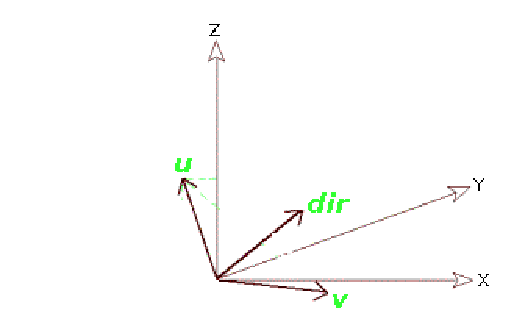
\includegraphics[scale=.8]{vectors.pdf}
\caption{The \tt{Alpha = 0} case. $X, Y, Z$ is the global coordinate system, $u$ is defined as being the vector orthogonal to the beam direction $dir$ and having the largest global $Z$ coordinate. $v$ is chosen such that $(dir, u, v)$ is a right-handed orthogonal basis. For a non-zero  \tt{Alpha} case, rotate $u$ and $v$ by \tt{Alpha} around $dir$}
\label{vectors}
\end{center}
\end{figure}

\paragraph{Optical components.}Available optics are semi-reflective mirrors, thin lenses (defined by their focal length and diameter), thick lenses (thickness on axis, refractive index, curvatures and diameter), and beam-dumps (which stop light). Optical components all have cylindrical symmetry, except for mirrors which may have a wedged face. The labeled "HR" surface is the principal surface, where beam are meant to be reflected or transmitted. In the case of mirrors it is the non-wedged surface. See section 4.1 for a list of available optical components and how to input their parameters.

Since mirrors can be wedged and do not have cylindrical symmetry, it is necessary to specify an angle to describe the position of the wedge in space. This is done in a similar fashion than in the beam case. If this angle (also called \tt{Alpha} is 0, then the point of the AR (wedged face) which is not affected by the wedging (it is the point on the rim of the original cylinder the AR was wedged from) has the largest global $Z$ component. Similarly as for beams, if the "maximum $Z$" condition makes no sense because the HR normal is  $+ e_Z$ (resp. $-e_Z$), then this reference point has largest (resp. smallest) $X$ coordinate.

If \tt{Alpha} is not 0, then this reference is situated at the image of the \tt{Alpha=0} reference point by the rotation of \tt{Alpha} around the normal (outpointing) vector of the HR surface. See figure \ref{cylinder} for an illustration.

\warn{On the contrary of lenses, the given center of the HR surface of mirrors on input is the center of the chord of the HR surface, and not the apex of the HR surface. Similarly, the thicknesses of mirrors as input are the thicknesses on the rim (rim of HR to closest point of wedged AR) and not on the optical axis.}

\begin{figure}[h]
\begin{center}
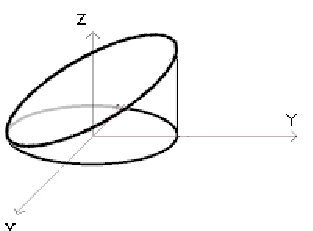
\includegraphics[scale=.8]{cylinder.pdf}
\caption{A mirror. Its center of HR is (0, 0, 0) and its normal to HR is $-e_Z$. Thus the reference point is (--1, 0, 0). Thus we can say that this is a thickness~=~0, positive wedged mirror with \tt{Alpha=}~225~$\degree$ (angle between the reference point and the point of the rim of the original cylinder which touches the AR face). Note that we could have also said a thickness~=~1, \textit{negatively} wedged mirror with \tt{Alpha=}~45~$\degree$.}
\label{cylinder}
\end{center}
\end{figure}


\subsection{Algorithm and approximations}
As previously described, \tt{theia} traces beams by interaction of the input beams with the optics, recursively. Here are the rules to calculate the beams.

\paragraph{Physical rules.}The laws of refraction and reflection are applied to calculate the directions of the new beams, as well as the origin $Q$ matrix (and the base vectors to express it) of the new beams.  The calculation of the $Q$ matrix follows a phase matching method and is detailed in \cite{1,2}. Total reflection is also taken into account, and the powers of the new beams are calculated according to the reflectance and transmittance of the surface. 

\warn{This rule introduces the approximation that the radius of curvature of the beam must be much smaller than the radii of curvature of the optics at hand. Apart from this, there are no other approximations (nor for the geometrical optics calculations to determine the direction of the new beams, nor for the exact point of origin of the new beams on the curved surfaces).}

\paragraph{Computational rules.}In order for the program to terminate, some computational rules have been introduced. Each simulation is led with an \textit{order} and a \textit{threshold}:

\begin{enumerate}
\item Each initial beam is created with a \textit{strayness order} of 0. Any beam reflected by a mirror AR face, transmitted by a mirror HR face, or reflected by any face of a lens has the order of its parent beam, plus one. Beams with an order larger than the simulation order are excluded from the following calculation step and their children are not determined. More generally, each surface of an optic has a certain action on the order of beams, depending on the nature (reflected or transmitted) of the beam and of the optic. For example, the surfaces of beam-splitters do not increase the order of beams, whereas all surfaces of lenses increase the order of reflected beams by 1, and those of transmitted beams by 0. See table \ref{actions} or the \textit{Quick Reference} document for a list of the actions of optics on beams.

\item The power of children beams are determined with the powers of the parent beams and the reflectance and transmittance of the surface. Similarly, beams with powers smaller than the simulation threshold are excluded from the following calculation step and their children are not determined.

\end{enumerate}

\begin{table}[h]
\begin{center}


\begin{tabular}{|p{1.5cm}|p{3.2cm}|p{3.2cm}|p{3.2cm}|p{3.2cm}|} \hline
\bf{Optic} & \bf{Action of ... HR on reflected} & \bf{HR on transmitted} & \bf{AR on reflected} & \bf{AR on transmitted } \\ \hline \hline
Mirror & +0 & +1 &+1 &+0 \\ \hline

Thick or thin lens & +1 & +0 & +0 & +1 \\ \hline

Beam-splitter & +0 & +0 & +0 & +0 \\ \hline

Special surface & User defined (see 4.1) & & & \\ \hline
\end{tabular}
\end{center}
\caption{The actions of surfaces of optical components on the strayness orders of beams}
\label{actions}
\end{table}

\section{Installation and usage}
\subsection{Installation instructions}
\tt{theia} uses the Python standard library component \tt{setuptools} to install the command line tool \tt{theia} as well as the Python library.

\paragraph{Local installation.}To install \tt{theia} to your local environment, \tt{cd} to the project repository root and issue the following commands:

\begin{itemize}
\item \tt{make install} to install the \tt{theia} command line program and library and compile the documentation in the \tt{doc/} sub-directory of the project;
\item \tt{make build-theia} to only install the program and the library but not compile the documentation (useful if you do not have a latex environment running);
\item \tt{make build-doc} to only compile the documentation (useful if you have modified the library to your liking --~please do).
\end{itemize}

\warn{This procedure will install the \tt{theia} script to \tt{\$HOME/.local/bin}, and this directory \textbf{must} be in your \tt{PATH} in order to have access to \tt{theia} from anywhere in your file system.}

\paragraph{System-wide installation.}For a system-wide installation, you can issue \tt{python setup.py install} with root privileges from the project root repository. The documentation must be compiled separately as indicated in the former paragraph and moved to some shared directory if you like.

\paragraph{Uninstalling.} Uninstalling a local installation if fairly simple: issue \tt{make clear} from the project root directory. This will wipe your \tt{\$HOME/.local} of anything that has to do with \tt{theia}. All the documentation, tutorial files or \tt{theia} input or output files elsewhere will of course stay in place after this procedure.

Uninstalling a system-wide installation is more tricky, and we do not provide an automated procedure for this and admins probably know better than us on this subject, though on most systems \tt{setuptools} puts library files in \tt{/usr/local/lib/python2.7/*-packages} and scripts in \tt{/usr/local/bin}.

\subsection{Usage on the command line}
The general usage of \tt{theia} is: \tt{theia [options] FNAME}, where:

\begin{itemize}
\item \tt{[options]} are command line options. See the next paragraph or the output of \tt{theia -h} for more details;
\item \tt{FNAME} is the name of the configuration file to use for the simulation, with or without the \tt{.tia} extension. See the next section for details on the format of the \tt{.tia} file.
\end{itemize}

\paragraph{Command line options.}As introduced in section 2. of this User Guide, \tt{theia} takes one configuration file as an input and may write out to output files and to standard output (the terminal window). The command line options allow the user to control all these outputs. The command line options are summed up in table \ref{option}.


\begin{table}[h]
\begin{center}
\begin{tabular}{| p{4cm} | p{10cm} |}
\hline
\textbf{Command line option} & \textbf{Effect} \\
\hline \hline
\tt{-h, --help} & Show the usage and the command line options of \tt{theia} and exit\\
\hline
\tt{-l FCLIB, --FreeCAD-lib FCLIB} & Specify\footnote{If you do not specify the location of the FreeCAD libraries on your system, \tt{theia} will try to find it itself, and issue an error if they were not found.} the location of the \tt{FreeCAD} libraries for the 3D visualization as being \tt{FCLIB} on your system\\
\hline
\tt{-i, --info} & During the simulation, do not output tracing information to standard output (see section 4.3 for details on the information that is output)\\
\hline
\tt{-w, --no-warn} & During the simulation, do not output warnings to standard output (see section 4.3 to find out what warnings may be written)\\
\hline
\tt{-t, --no-text} & After the simulation, do not write the \tt{.out} text output file (see section 4.2 for details)\\
\hline
\tt{-c, --no-CAD} & After the simulation, do not write the CAD file\\
\hline
\tt{-a, --anti-clipping} & Include anti-clipping in simulation (see next paragraph) \\
\hline
\tt{-s, --short-output} & Exclude beams propagating inside optics from text output, terminal output and CAD rendering files. This also changes the way beams are referenced to in these files and in the terminal output\\
\hline
\tt{-v, --version} & print version of \tt{theia} and exit\\
\hline
\end{tabular}
\end{center}
\caption{Command lines options of \tt{theia}.}
\label{option}
\end{table}

\paragraph{Note on anti-clipping.}Anti-clipping is when a beam passes near an optic without formally interacting but its axis is within 2 waists of the optic. This leads to power losses and diffused light. It is the opposite of clipping, in which the beam is not completely included in the optic it is interacting with.

Warnings are always issued when clipping occurs (except if the \tt{-w, --no-warn} option is used), but calculations for anti-clipping are heavier (they add approximately half more tracing calculations), and are only done if the \tt{-a, --anti-clipping} option is used. If it is, then corresponding warnings are issued.

\paragraph{Note on the \tt{FreeCAD} libraries.}\tt{theia} writes the 3D visualization information for the simulation to a CAD file to be read by \tt{FreeCAD}. If you do not wish to write the CAD file or if you do not have the \tt{FreeCAD} libraries installed, you may use the \tt{-c} command line option.

On the contrary, if you have the \tt{FreeCAD} libraries and you know where they are (usually \tt{usr/lib/freecad/lib}), you can save \tt{theia} the effort of finding them by aliasing \tt{theia} with \tt{theia -l [WHERE YOUR FREECAD LIB IS]}.


\section{Input and output to theia}
\subsection{The \tt{.tia} input format}
\tt{.tia} format input files are simple text files reporting the simulation parameters and the optical setup to the \tt{theia} CLI tool. In such a file, each line is used to describe its own object\footnote{By the way, all spaces and tabs are ignored, so you can throw some in wherever you want.}. These objects can be simulation parameters, simulation meta-data or optical components. The object you are specifying with a given line depends on the format of the line, according to the following table \ref{inputformat}.

\begin{table}[h]
\begin{center}
\begin{tabular}{|p{3cm}|p{4cm}|p{8cm}|}
\hline
\textbf{Lines starting with ...} & \textbf{... specify ...} & \textbf{... and the rest of the line is ...} \\ \hline \hline

\tt{\#} & a comment & ignored \\ \hline

\tt{order=} & the order of the simulation & a Python expression evaluating to an integer \\ \hline
\tt{threshold=} & the threshold of the simulation & a Python expression evaluating to a floating point number  \\ \hline
\tt{bo} & the coordinates of an optical bench, i.e a new reference for coordinates (these coordinates will be added to the optics specified after this line and until the next \tt{bo}  line) & a comma-separated list of \textit{entries} specifying the origin of the bench \\ \hline
\tt{bm} & an input orthogonal Gaussian beam & a comma-separated list of \textit{entries}  (see following paragraph) specifying the characteristics of the beam \\ \hline
\tt{mr} & a mirror object & a comma-separated list of \textit{entries} specifying the characteristics of the mirror \\ \hline
\tt{bs} & a beam-splitter object & a comma-separated list of \textit{entries} specifying the characteristics of the beam-splitter \\ \hline
\tt{sp} & a special optic object (of which the user specifies explicitly the actions of surfaces on beam orders) & a comma-separated list of \textit{entries} specifying the characteristics of the optic \\ \hline
\tt{th} & a thinlens object & a comma-separated list of \textit{entries} specifying the characteristics of the thin lens \\ \hline
\tt{tk} & a thicklens object & a comma-separated list of \textit{entries} specifying the characteristics of the thick lens \\ \hline
\tt{bd} & a beamdump object (which stops all beams) & a comma-separated list of \textit{entries} specifying the characteristics of the beamdump \\ \hline
\tt{gh} & a ghost surface (which does not affect the beam but only make a new entry in the \tt{.out} file) & a comma-separated list of \textit{entries} specifying the characteristics of the ghost surface \\ \hline

anything else & the long name of the simulation (appears in the output file) & any text input (spaces and tabs will be stripped) \\ \hline



\end{tabular}
\end{center}
\caption{Format of each type of line in a \tt{.tia} input file}
\label{inputformat}
\end{table}

For beams, mirrors, beam-splitters, special surfaces, beamdumps, ghost surfaces, thin and thick lenses, report to the \textit{Quick Reference} document in order to know what are the order and the signification of the entries.

\paragraph{Entries and available Python expressions.}An entry in a input file line is of the form (remember spaces and tabs are not taken into account) \tt{VAR=EXPRESSION} or simply \tt{EXPRESSION}. Use the second form when you have specified all the parameters since the beginning of the line and in the right order, and the first form when you want to input in the order you like, or you have omitted some parameters (think of this as a set of argument to a function, the arguments are considered in the right order and complete until the first \tt{VAR=EXPRESSION}, and then its up to you to specify or not the following parameters).

\tt{EXPRESSION} is any Python expression that is valid \textit{in the scope where the input reading function is defined}. What this means is that you can use:
\begin{itemize}
\item Standard Python literal integers, floats and operators: \tt{4.}, \tt{.2e-3 * 3 / 2}, etc.
\item The functions and constants that are available as built-ins in this scope (these are listed in the \textit{Quick Reference} document): \tt{arccos(3 * exp(-2.)) * mW}, \tt{sqrt(4.*mm*mm)}, \tt{arctan(pi/12)}, etc.
\item Any user defined function or constant as long as it is declared as a global in the \\ \tt{theia.helpers.settings} module and initialized correctly (see section 5.1 on globals), declared in the \tt{theia.helpers.units} module, or declared directly in \tt{theia.running.parser}. After all of these operations, \tt{theia} has to be rebuilt with \tt{make install}.
\end{itemize}




\warn{As we just mentioned, the parts of an entry line which are between two commas or between a comma and a \tt{=} sign are evaluated as Python expressions, which allows for a great flexibility of the input. \textit{Nonetheless}, you must beware of Python expressions evaluation which might lead to unexpected behavior, particularly on integers! For example, if one enters \tt{(3/4)*pi}, the evaluation will lead to 0 because of integer division, and not $3\pi/4 = 135\degree$. To obtain $135\degree$, one should enter \tt{3*pi/4}, or \tt{(3./4)*pi} for instance.}



\paragraph{Empty constructors.}In \tt{theia}, all the constructors available to the user have a complete set of default values (see section 5.2 for details on this). Thus an input file can very well contain a line with a tag and \textit{zero} arguments, such as:

\tt{\#example usage of a empty constructor for a (thus default) input beam}

\tt{bm}


To find out what the default values of all the constructors are, report to the \textit{Quick Reference} document.


\paragraph{Meta data-specifying lines overwrite each other.}Lines used to specify the simulation order, threshold and long name overwrite each other. If you specify a "\tt{threshold=}" line after another "\tt{threshold=}" line, this latter one will overwrite the value specified in the former line. The same mechanics apply to "\tt{order=}" and long-name lines.

\subsection{The \tt{.out} output file}
The output file is also a simple text file. In contains formatted information on the simulation, the optics present in the setup and the beams generated by these. All this information is divided in sections:

\begin{itemize}
\item The \tt{META DATA} section specifies the date at which the file was written, the input file used, the various simulation parameters.

\item The \tt{SIMULATION DATA} section gives information on the components used in the simulation (component type, reference and position of the HR surface chord center), and on the generated beam trees (a reference to their original beam and the number of beams the tree contains in total).

\item The \tt{BEAM LISTING} section reports, in a beam tree by beam tree fashion, the beams  contained in the different beam trees. for each beam, you will find the optic and face the beam departs from, the length of the beam, the optic and face the beam finishes on, the reference to the beam, and then the waist positions (along the beam starting from the beam origin), waist sizes and finally beam direction. The waists are given in the proper basis attached to the beam, as described in section 2.3.
\end{itemize}

\paragraph{Beam references.}The reference of each beam (as it appears at the end of each entry in the \tt{BEAM LISTING} section of the output file) is the reference of its parents beam plus a tag which can be \tt{r} or \tt{t} according to whether the beam was produced by reflexion or transmission of the parent beam. The references of the input beams are read in the input file.


Here is a sample of output:\\

\tt{(M1, AR) 0.946496969941m (L1, HR) TBttt \{}

	\quad	\tt{Waist Pos: (-1.8387309993210437, -1.8387309993210468)m}

	\quad	\tt{Waist Size: (0.00016310752802, 8.15537640098e-05)mm}

	\quad	\tt{Direction: (90.0, 4.68099236149e-13)deg}

	\tt{\}}\\

This sample describes a beam traveling 94.6~cm from the AR surface of the optic labeled M1 (surely a mirror) to the HR surface of the optic labeled L1 (surely a lens). This beam is the beam transmitted by the beam transmitted by the beam transmitted by the input beam labeled \tt{TB}. It waists are about .1~$\mu$m and both located 1.83~m behind the origin of the beam (thus this beam is in its diverging phase all the way from M1 to L1). Its direction is along the positive $X$ axis.

\paragraph{Note on short beam references}.The default way of referencing beams (appending \tt{r} or \tt{t} at every interaction) can produce very heavy beam references in the case of a large simulation. Thus, a command line option \tt{-s, --short-output} is provided. When this option is used:

\begin{enumerate}
\item Only the beams propagating \textit{outside} the optics will be reported to the output files (text and CAD)
\item All the references to the beams are shortened in the following manner: instead of using \tt{r} and \tt{t} to indicate reflection and transmission on \textit{surfaces} of optics, \tt{R} and \tt{T} are used to signify reflection and transmission on \textit{optics as a whole}. For example, a reference \tt{ttrtt} corresponds to two transmissions, a reflection and again two transmissions, which in turn corresponds to being transmitted globally by an optic, then reflected, then transmitted, given that input beams are (generally) outside of optics, and thus the short reference of such a beam will be \tt{TRT}, which is simpler. We may say of this beam that it was transmitted by the first optic it encountered, then reflected by the next and transmitted by the next. 
\end{enumerate}


\subsection{The \tt{.fcstd} output file}

\tt{theia} writes the 3D visualization information to a \tt{.fcstd} file to be read by the free software \tt{FreeCAD}. This file is intended to ease navigation in the optical setup and also to review the characteristics of the traced beams.

Once the simulation is done, open the \tt{.fcstd} file with \tt{FreeCAD}. Every simulation object (beam, optic, etc.) has one CAD object associated to it, these are all listed in the left panel of the \tt{FreeCAD} window. These objects contain all the relevant optical and geometrical data on the simulation objects. Of course, all these objects can be manipulated with the CAD software.

See figure \ref{shot} for an example of the 3D viewing.

\begin{figure}[h]
\begin{center}
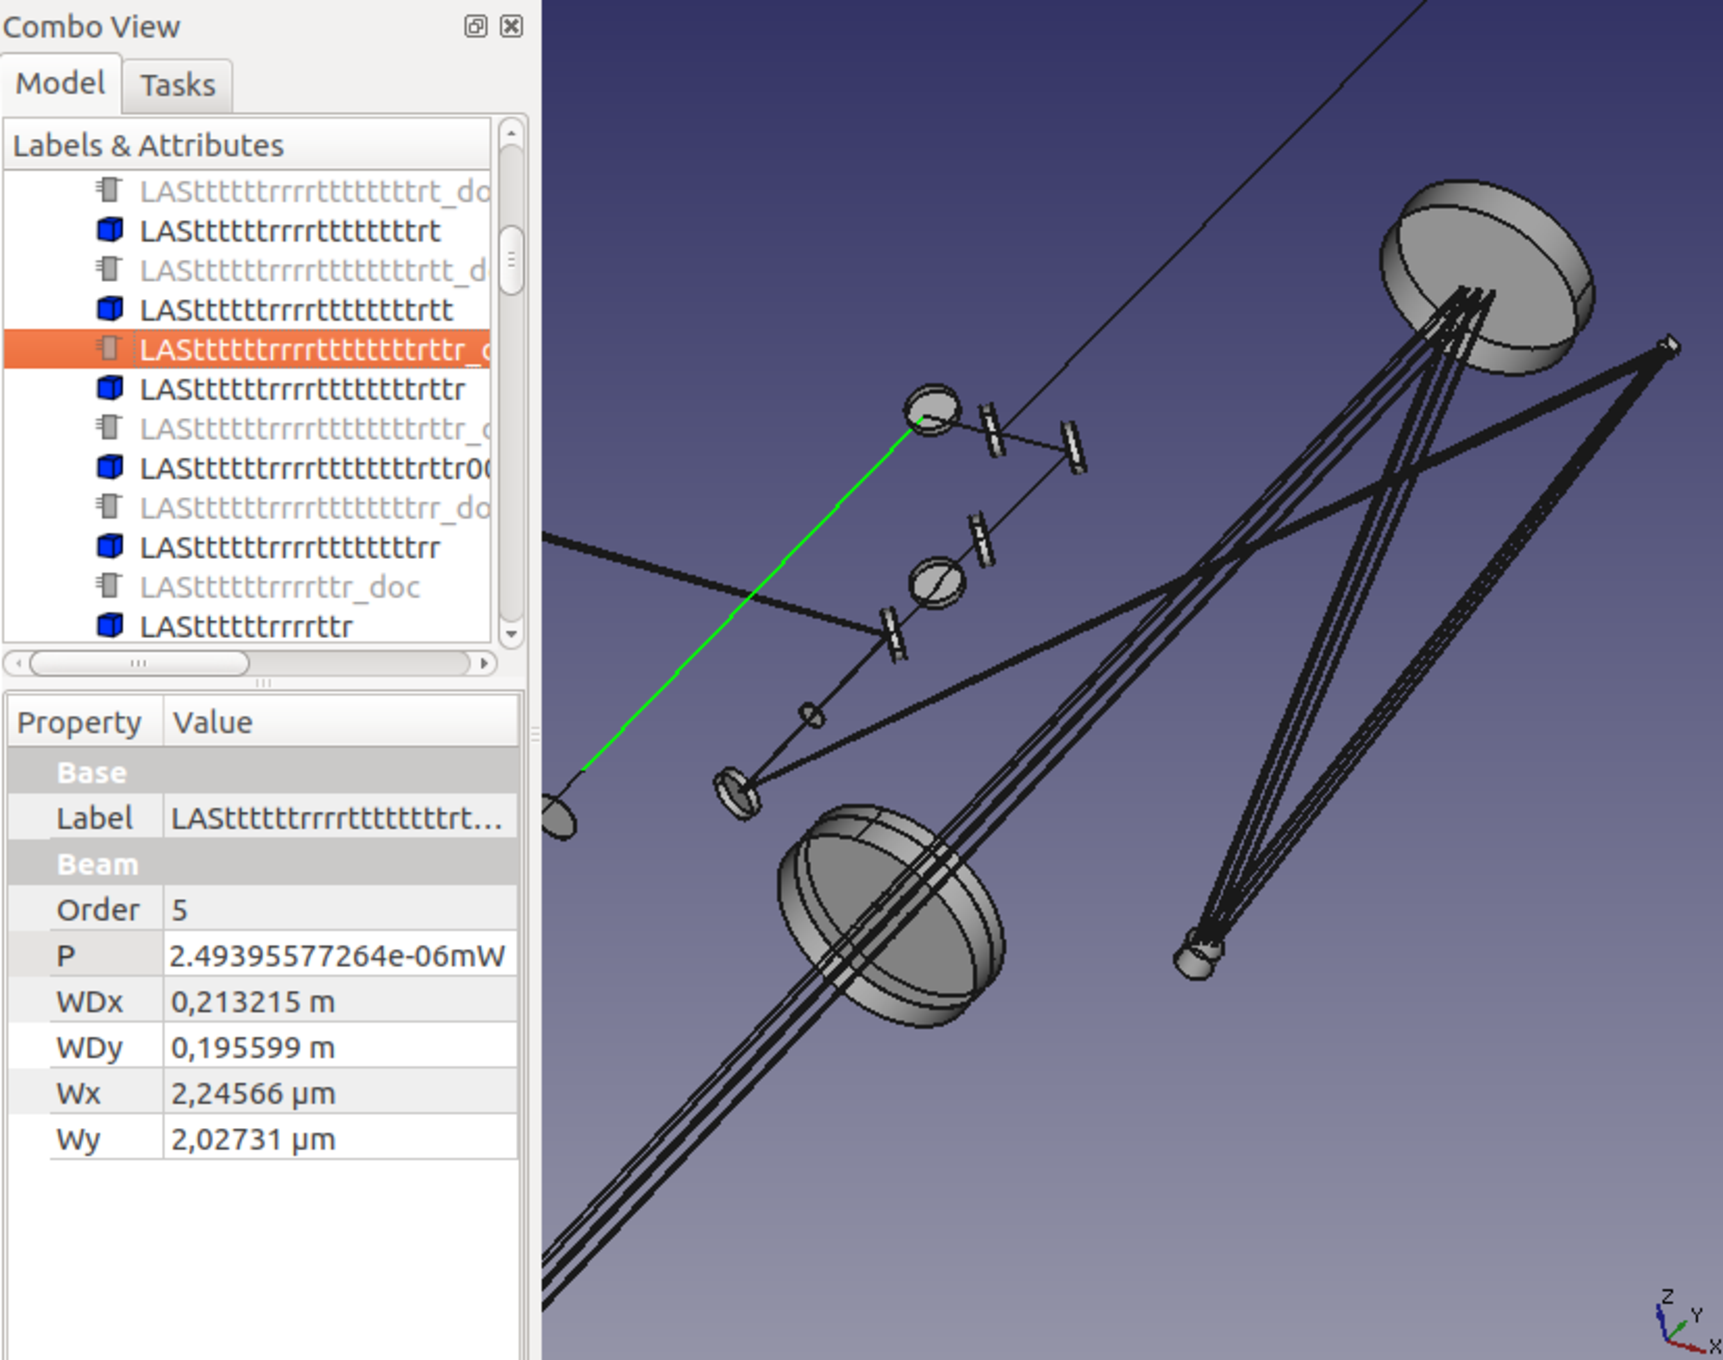
\includegraphics[scale=.4]{shot}
\end{center}
\caption{The 3D viewer reading the \tt{.fcstd} file of \tt{theia}. On the left panel, one sees a beam object (which was highlighted when the beam on the view was clicked on by the user) and the corresponding Gaussian and geometrical data of the beam.}
\label{shot}
\end{figure}


\newpage
\section{An introduction to the theia API}

This section is an introduction to the Application Programmers Interface to the \tt{theia} library. It give somewhat more detail on the algorithm and data structures of theia and how they are implemented in \tt{theia}. This guide may be useful to anyone who wants to use \tt{theia} to develop their own optical simulation scripts, and to anyone who would like to contribute to \tt{theia}. For a through and complete treatment of the \tt{theia} API, see the \textit{API Guide} document or the online documentation.

Throughout this section, Unix \tt{paths/like/this} are understood as relative to the theia project root directory (\textit{e.g.} \tt{doc/img/flow.png}) and Python import statements \tt{like.this.one} are understood as relative to the theia package (\textit{e.g.} \tt{running.simulation.Simulation.\_\_init\_\_}).


\subsection{A note on global variables}
The \tt{theia} CLI tool uses a certain number of global variables in order to keep values which don't change along the execution. These global variables are consequently needed by a certain number of functions defined in the library in order for the CLI tool to be as functional as possible. When using \tt{theia} as a library, one may not need all these globals and they may even get in the way of development.

\paragraph{How to take care of the globals once and for all.}The global variables are \textit{all} declared in \tt{helpers.settings} and are initialized with \tt{helpers.settings.init} at the very beginning of \tt{main.main}, which takes in a dictionary and reads the globals from there. If you don't want to hear about the globals, you can place the following snippet (found in \tt{tests/test\_simulation.py}) at the beginning of your script and not worry about the globals.

\begin{lstlisting}
# use this snippet and all globals worries are gone
from theia.helpers.settings import init

# initialize globals in a dictionary
dic = {'info': True, 'warning': True, 'text': True, 'cad': True,
       'fname': 'theiasimulation', 'fclib': '/usr/lib/freecad/lib',
       'antiClip': True, 'short': False}

init(dic)

# you're all set
\end{lstlisting}

\paragraph{Who uses the globals?}Here is a table (table \ref{globals}) listing the global variables and which functions use them.

\begin{table}[h]
\begin{center}

\begin{tabular}{|c | l |}
\hline
\textbf{Global} & \textbf{Used by} \\ \hline \hline

\tt{info} & \tt{optics.beamdump.BeamDump.hit} \\
& \tt{optics.optic.Optic.hitHR} \\
& \tt{optics.optic.Optic.hitAR} \\
& \tt{optics.optic.Optic.hitSide} \\
& \tt{tree.beamtree.treeOfBeam} \\ \hline

\tt{warning} & \tt{optic.mirror.Mirror.\_\_init\_\_} \\
&\tt{optic.beamsplitter.BeamSplitter.\_\_init\_\_} \\
&\tt{optic.special.Special.\_\_init\_\_} \\
& \tt{optic.thicklens.ThickLens.\_\_init\_\_} \\
& \tt{optic.thinlens.ThinLens.\_\_init\_\_} \\
& \tt{running.simulation.Simulation.run} \\
& \tt{tree.beamtree.treeOfBeam} \\ \hline

\tt{text, cad, fclib} & \tt{main.main} \\ \hline

\tt{fname} & \tt{main.main} \\
& \tt{running.simulation.Simulation.load} \\
& \tt{running.simulation.Simulation.writeOut} \\
& \tt{running.simulation.Simulation.writeCAD} \\ \hline

\tt{antiClip} & \tt{tree.beamtree.treeOfBeam} \\ \hline
\tt{short} & \tt{optics.beamdump.BeamDump.hit} \\
& \tt{optics.Optic.hitHR} \\
& \tt{optics.Optic.hitAR} \\
& \tt{optics.Optic.hitSide} \\
& \tt{rendering.writer.writeTree} \\
& \tt{running.simulation.Simulation.writeOut} \\
& \tt{tree.beamtree.BeamTree.lines} \\
& \tt{tree.beamtree.BeamTree.outputLines} \\
& \tt{tree.beamtree.treeOfBeam} \\ \hline

\end{tabular}
\caption{The global variables of theia and the functions who use them}
\label{globals}
\end{center}
\end{table}
\subsection{Classes and inheritance hierarchy}
Figure \ref{inheritancehierarchy} presents the inheritance hierarchy of the classes of \tt{theia}.

\begin{figure}[h]
\begin{center}
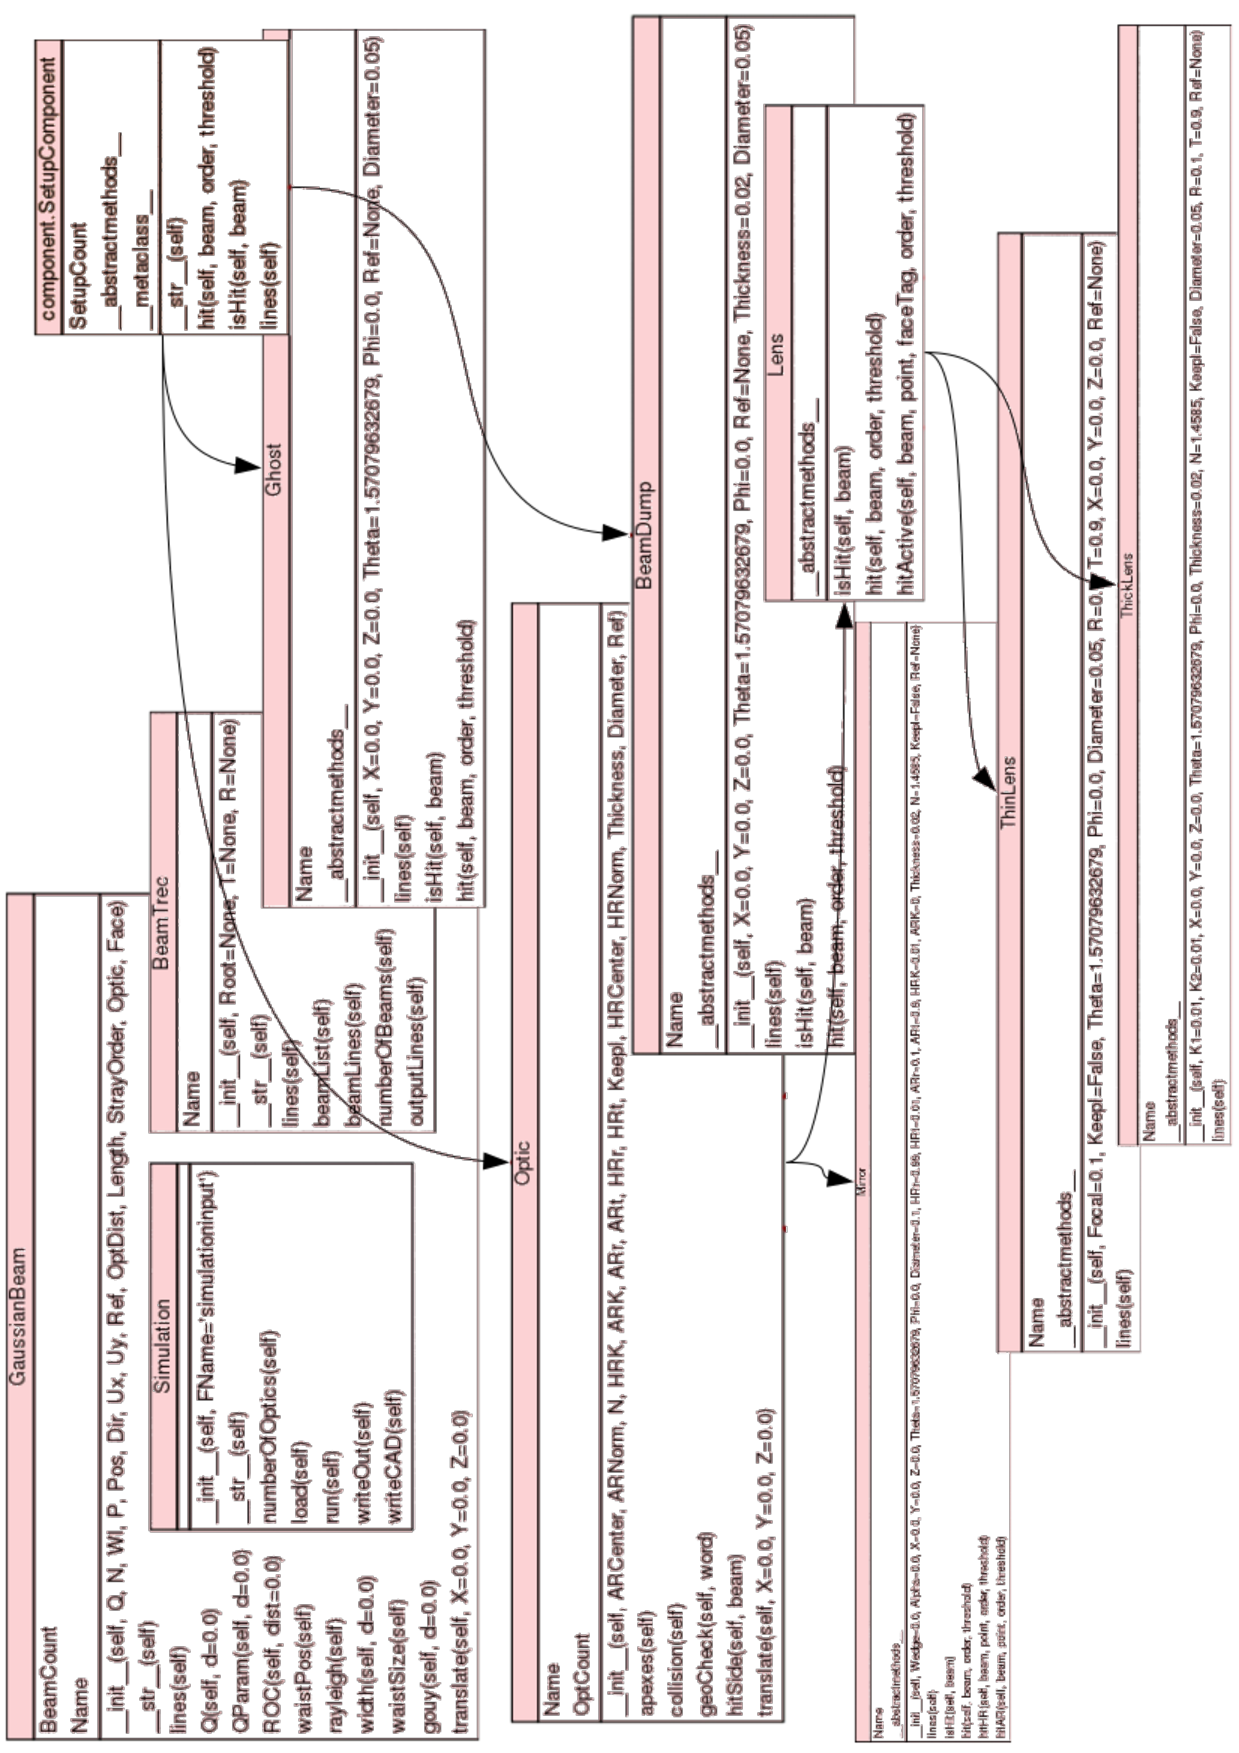
\includegraphics[scale=.3]{inheritancehierarchy.pdf}
\caption{Inheritance hierarchy of theia}
\label{inheritancehierarchy}
\end{center}
\end{figure}
\paragraph{A word on initializer default values.}We try to avoid surprises and stay consistent throughout the code with the following policies concerning classes at the leaves of the inheritance graph:

\begin{enumerate}
\item For classes whose initializers will be called only with input form users (read from an input file or in a script), \textit{every} parameter of the constructor has a default value and the constructor can be called \textit{without arguments}. What's more, the input of the user is processed through the class initializer and then fed to the initializer of the mother class. For example, the user may provide \tt{X}, \tt{Y} and \tt{Z} to the constructor she or he calls, then these are processed and it is \tt{[X, Y, Z]} as a list (with types checked etc.) which is fed to the mother initializer.

\item For classes whose initializers are called solely internally, there are \textit{no default values}. These are the constructors of \tt{SetupComponent}, \tt{Optic}.

\item For classes that may be instantiated internally and by users, the module defining the class defines a global scope function, whose parameters \textit{all have default values} and which is intended to be used with input from the user, as the constructors described in the previous point 1. This function is named \tt{user\$CLASSNAME} and processes the input of the user into input for the class's proper \tt{\_\_init\_\_} initializer. On the other hand, this proper initializer is intended for internal use only and has \textit{no default values}. This is for example the case of the \tt{optics.beam.GaussianBeam} class, whose constructor is called internally to generate new beams and with user input read from the input file. In this last case it is \tt{userGaussianBeam} which is called.
\end{enumerate}

\paragraph{Abstract Base Classes.}The highest class of the optical classes hierarchy is the \\ \tt{optics.component.SetupComponent} class. Its metaclass is set to \tt{abc.ABCMeta}, making it an abstract base class\footnote{See \tt{docs.python.org/2/library/abc.html} for details}. This essentially means that no daughter class of this class can be instantiated unless all the methods decorated with \tt{abc.abstractmethod} have been reimplemented by the daughter class. The methods concerned with this limitation are \tt{optics.component.SetupComponent.lines} and \tt{optics.component.SetupComponent.isHit}. Methods decorated with \tt{abstractmethod} in an abstract base class can eventually be implemented in the mother class, but in theia they all \tt{pass}, and could be called \textit{pure virtual} for someone coming from C++.

\subsection{Call graph}
Here (figure \ref{callgraph}) is the call graph of the \tt{theia} CLI tool, from which one can easily deduce the call graph of any individual function. You can refer to the \textit{API Guide} or the online API documentation to find out in which module the functions are defined.


\begin{figure}[h]
\begin{center}
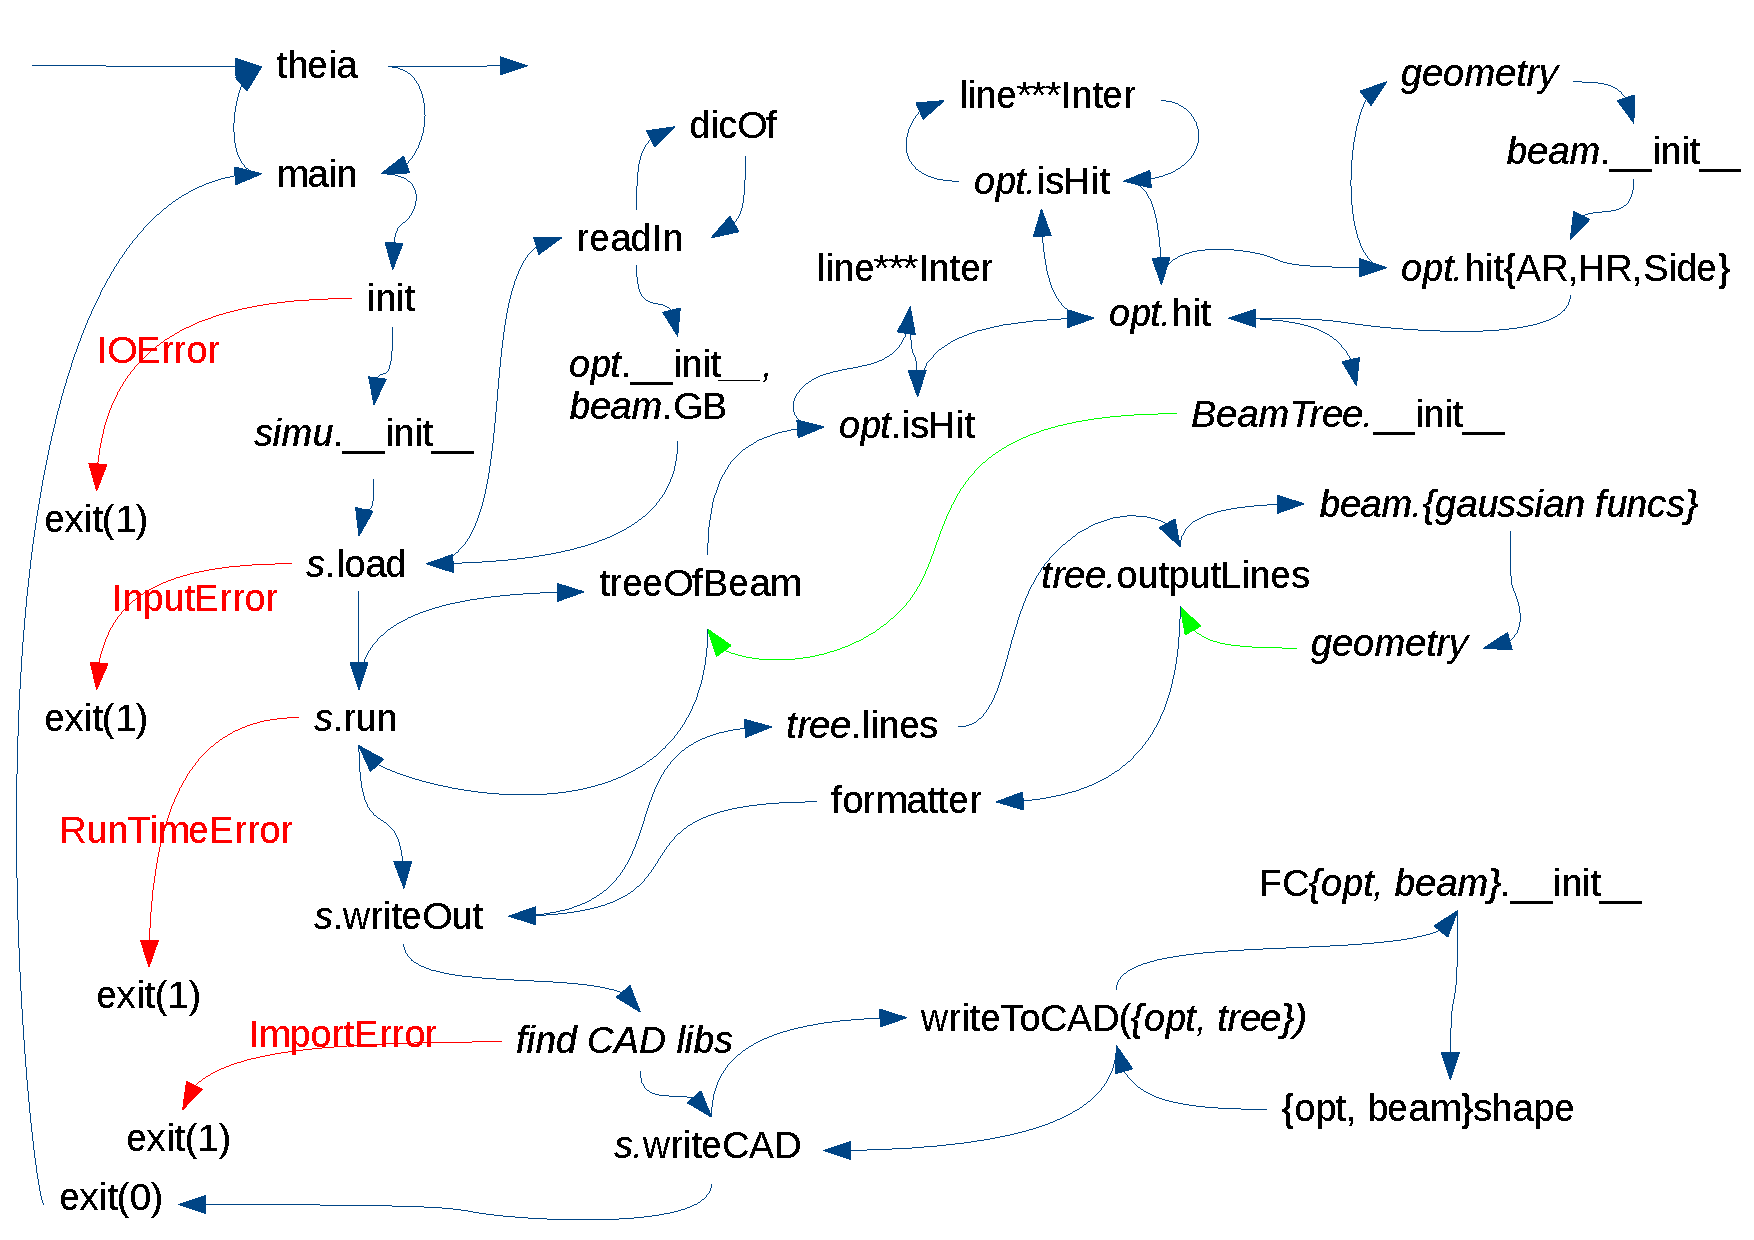
\includegraphics[scale=.5]{callgraph.pdf}
\end{center}
\caption{Call graph of the \tt{theia} CLI tool. \textit{italics}: generic object or group of methods, \textcolor{green}{green:} recursive call, \textcolor{red}{red:} handled exception.}
\label{callgraph}
\end{figure}



\paragraph{Note on the  call stack.}According to this call graph (figure \ref{callgraph}), the stack has a maximum height of $9~+~2(n-1)$ when there are $n$ levels of recursion. Generally, the program crashes --~if it crashes~-- by recursion depth limit exceeding (leading to a handled \tt{RunTimeError} exception and an exit with an error code of 1) before causing a stack overflow.

\subsection{Miscellaneous remarks}

\paragraph{Coding style.}In the development of \tt{theia} we have tried to stick to a couple of coding style conventions, which may help to review the code and are important to know for anyone wishing to contribute.

\begin{itemize}
\item The code of \tt{theia} is heavily commented and doc-stringed, and it should stay that way in order for \tt{theia} to be an accessible library.

\item Throughout the library, classes and attributes look \tt{LikeThis} whereas objects and methods look \tt{likeThis}.

\item There is an approximate \textit{one file} $\rightarrow$ \textit{one class} correspondence and files are named accordingly with the objects they define. Generally, we have a tendency to distribute functions in different modules if they provide different functionalities, regardless of the total number of modules. Functions are together in a module if they belong together, consequently they are many modules in theia.

\item We tend never to skip more than 1 line (Python is already very formatted).

\item \tt{\# Provides} lines at the very beginning of modules allow to know at a glance what variables, functions and classes the module provides.

\item Imports: import first from the Python standard library and third-party packages, then from \tt{theia} sub-packages other than the current, then from the current \tt{theia} sub-package. For \tt{theia} sub-packages imports, always use the \tt{from ... import} idiom, always use relative imports (\tt{from ..helpers import interaction}) and for standard library and third-parties always \tt{import} before you \tt{from ... import}. We try to not import what we don't need.

\item Class doc-string: present class attributes before instance attributes and mention if they are inherited.
\end{itemize}

\paragraph{Writing to \tt{stdout} and files.}Many classes reimplement the \tt{\_\_str\_\_} method to have \tt{print(object)} print a neatly formatted description of the object. To this effect there are two important methods: \tt{lines} (instance method) and \tt{helpers.tools.formatter} (global scope function). \tt{formatter} takes a list of strings (lines to output) and makes C-style indented output with curly braces in the right place in one large string. Basically, one has:

\begin{lstlisting}
# inside class scope
def __str__(self):
	return formatter(self.lines())

\end{lstlisting}

\begin{thebibliography}{99}

\bibitem{1}
Kochkina, Wanner, Schmelzer, Tr\"obs, Heinzel:
\textit{Modeling of the General Astigmatic Gaussian Beam and its Propagation through 3D Optical Systems},
Applied Optics 24 (2013)

\bibitem{2}
Arnaud, Kogelnik:
\textit{Gaussian Light Beams with General Astigmatism},
Applied Optics 8 (1969)

\end{thebibliography}

\end{document}
